% Define document class
%\documentclass[twocolumn,twocolappendix,linenumbers]{aastex631}
\documentclass[modern,linenumbers]{aastex631}
% Some entries inspired from a preamble by Adrian Price-Whelan, https://github.com/adrn/PhaseSpiralAsteroseismology/blob/main/tex/preamble.tex

\usepackage{showyourwork}

% Latex imports
\let\tablenum\relax             % necessary for AASTeX
\usepackage{siunitx}
\sisetup{range-phrase= \text{--}, range-units=single, separate-uncertainty=true}
\sisetup{separate-uncertainty=true}
\usepackage{blindtext}          % Filler text
\usepackage{xcolor}
\usepackage[T1]{fontenc}

\usepackage[toc,nogroupskip,nohypertypes={glossary}]{glossaries} % import after hyperref
\glsdisablehyper

\newglossaryentry{HST}{name={HST}, description={Hubble Space Telescope}, first={Hubble Space Telescope (HST)}}
\newglossaryentry{NIR}{name={NIR}, description={Near-Infrared}, first={near-infrared (NIR)}}
\newglossaryentry{MIR}{name={MIR}, description={Mid-Infrared}, first={mid-infrared (MIR)}}
\newglossaryentry{FIR}{name={FIR}, description={Far-Infrared}, first={far-infrared (FIR)}}
\newglossaryentry{FUV}{name={FUV}, description={Far-Ultraviolet}, first={far-Ultraviolet (FUV)}}
\newglossaryentry{NUV}{name={NUV}, description={Near-Ultraviolet}, first={near-Ultraviolet (NUV)}}
\newglossaryentry{EUV}{name={EUV}, description={extreme-Ultraviolet}, first={extreme-Ultraviolet (EUV)}}
\newglossaryentry{SED}{name={SED}, description={Spectral energy distribution}, first={spectral energy distribution (SED)}, firstplural={spectral energy distributions (SEDs)}}
\newglossaryentry{ppm}{name={ppm}, description={parts per million}, first={parts per million (ppm)}}
\newglossaryentry{PDF}{name={PDF}, description={Probability density function}, first={probability density function (PDF)}, firstplural={probability density functions (PDF)}}
\newglossaryentry{PLATO}{name={PLATO}, description={PLAnetary Transits and Oscillations of stars}, first={PLATO~\citep[][]{Rauer2014}}}
\newglossaryentry{PSF}{name={PSF},description={Point Spread Function}, first={point spread function (PSF)}, firstplural={point spread functions (PSF)}}
\newglossaryentry{SFD}{name={SFD}, description={Size frequency distribution}, first={size frequency distribution (SFD)}, firstplural={Size frequency distributions (SFD)}}
\newglossaryentry{SNR}{name={SNR}, description={Signal-to-noise ratio}, first={signal-to-noise ratio (SNR)}}
\newglossaryentry{RV}{name={RV}, description={Radial Velocity}, first={Radial Velocity (RV)}, firstplural={Radial Velocities (RV)}}
\newglossaryentry{TTV}{name={TTV}, description={Transit Timing Variation}, first={transit timing variation (TTV)}, firstplural={transit timing variations (TTVs)}}
\newglossaryentry{TESS}{name={TESS}, description={Transiting Exoplanet Survey Satellite}, first={Transiting Exoplanet Survey Satellite~\citep[\textit{TESS},][]{Ricker2014}}}
\newglossaryentry{TIC}{name={TIC}, description={\textit{TESS} Input Catalog}, first={\textit{TESS} Input Catalog~\citep[TIC,][]{Stassun2018}}}
\newglossaryentry{JWST}{name={JWST}, description={James Webb Space Telescope}, first={James Webb Space Telescope~\citep[\textit{JWST},][]{Beichman2014}}}
\newglossaryentry{HZ}{name={HZ}, description={habitable zone}, first={habitable zone (HZ)}}
\newglossaryentry{EEC}{name={EEC}, description={exo-Earth candidate}, first={exo-Earth candidate (EEC)}, firstplural={exo-Earth candidates (EEC)}}
%\newglossaryentry{}{name={}, description={}, first={}, firstplural={}}


% package to open file containing variables
\usepackage{datatool, filecontents}
\DTLsetseparator{,}% Set the separator between the columns.

% import data
\DTLloaddb[noheader, keys={thekey,thevalue}]{variables}{variables.dat}
% Loads variables.dat with column headers 'thekey' and 'thevalue'
\newcommand{\var}[1]{\ensuremath{\DTLfetch{variables}{thekey}{#1}{thevalue}}}

% paper comments
\usepackage{comment}						 % comments that can be switched visible/invisible
\includecomment{comment}
%\specialcomment{outtake}{\begingroup\sffamily\color{gray}}{\endgroup}
%\specialcomment{note}{\begingroup\sffamily\color{red!40!green!70!blue!90}}{\endgroup}
\specialcomment{note}{\begingroup\sffamily\color{gray}}{\endgroup}
%\excludecomment{note}                       % switch notes off

%% switch TODO notes on/off
\usepackage[backgroundcolor=red!20!green!40!blue!10, textsize=tiny]{todonotes}
% \usepackage[disable]{todonotes}			% switches all todo notes to invisible
\usepackage{regexpatch}
\makeatletter
\xpatchcmd{\@todo}{\setkeys{todonotes}{#1}}{\setkeys{todonotes}{inline,#1}}{}{}
\makeatother

%% manuscript revision
%\newcommand{\rev}[1]{{\textbf{#1}}}    % on
\newcommand{\rev}[1]{{#1}}              % off

%% ... and second revision
\newcommand{\revv}[1]{{\textbf{#1}}}    % on
%\newcommand{\revv}[1]{{#1}}            % off

% ---------------------------------
% PAPER VARIABLES

% ---------------------------------
% CONSTANTS/MISSIONS/ABBREVIATIONS

% SIunitx definitions
\DeclareSIUnit\mSun{M_\odot}
\DeclareSIUnit\Msun{M_\odot}
\DeclareSIUnit\mStar{M_\star}
\DeclareSIUnit\Mstar{M_\star}
\DeclareSIUnit\mEarth{M_\oplus}
\DeclareSIUnit\Mearth{M_\oplus}
\DeclareSIUnit\rEarth{R_\oplus}
\DeclareSIUnit\Rearth{R_\oplus}
\DeclareSIUnit\year{yr}
\DeclareSIUnit\au{au}
\DeclareSIUnit\dex{dex}
\DeclareSIUnit\ppm{ppm}
\DeclareSIUnit\eV{eV}
\DeclareSIUnit\parsec{pc}
\DeclareSIUnit\photons{photons}
\DeclareSIUnit\erg{erg}

% Missions/Projects/Packages
\newcommand{\code}[1]{\texttt{#1}}
\newcommand{\project}[1]{\textsl{#1}}

\newcommand{\bioverse}{\code{Bioverse}}
\newcommand{\emcee}{\project{emcee}}

\newcommand{\rst}{\project{Nancy Grace Roman Space Telescope}}
\newcommand{\plato}{\project{PLATO}}
\newcommand{\cheops}{\project{CHEOPS}}
\newcommand{\kepler}{\project{Kepler}}
\newcommand{\ktwo}{\project{K2}}
\newcommand{\tess}{\project{TESS}}
\newcommand{\ariel}{\project{Ariel}}
\newcommand{\nautilus}{\project{Nautilus}}
\newcommand{\life}{\project{LIFE}}
\newcommand{\hwo}{\project{Habitable Worlds Observatory}}
\newcommand{\gclef}{\project{G-CLEF}}
\newcommand{\gmt}{\project{Giant Magellan Telescope}}
\newcommand{\andes}{\project{ANDES}}
\newcommand{\elt}{\project{European Extremely Large Telescope}}
\newcommand{\modhis}{\project{MODHIS}}
\newcommand{\tmt}{\project{Thirty Meter Telescope}}
\newcommand{\gaia}{\project{Gaia}}

% Stats / probability
\newcommand{\given}{\,|\,}
\newcommand{\norm}{\mathcal{N}}
\newcommand{\pdf}{\textsl{P}}
%\newcommand{\GG}{\mathbb{G}}
%\newcommand{\pbio}{\mathrm{}}

% Maths
\newcommand{\dd}{\mathrm{d}}
\newcommand{\transpose}[1]{{#1}^{\mathsf{T}}}
\newcommand{\inverse}[1]{{#1}^{-1}}
\newcommand{\argmin}{\operatornamewithlimits{argmin}}
\newcommand{\mean}[1]{\left< #1 \right>}

% Non-scalar variables
\renewcommand{\vec}[1]{\ensuremath{\bs{#1}}}
\newcommand{\mat}[1]{\ensuremath{\mathbf{#1}}}

% Unit shortcuts
\newcommand{\msun}{\ensuremath{\mathrm{M}_\odot}}
\newcommand{\mjup}{\ensuremath{\mathrm{M}_{\mathrm{J}}}}
\newcommand{\kms}{\ensuremath{\mathrm{km}~\mathrm{s}^{-1}}}
\newcommand{\mps}{\ensuremath{\mathrm{m}~\mathrm{s}^{-1}}}
\newcommand{\pc}{\ensuremath{\mathrm{pc}}}
\newcommand{\kpc}{\ensuremath{\mathrm{kpc}}}
\newcommand{\kmskpc}{\ensuremath{\mathrm{km}~\mathrm{s}^{-1}~\mathrm{kpc}^{-1}}}
\newcommand{\dayd}{\ensuremath{\mathrm{d}}}
\newcommand{\yr}{\ensuremath{\mathrm{yr}}}
\newcommand{\AU}{\ensuremath{\mathrm{AU}}}
\newcommand{\Kel}{\ensuremath{\mathrm{K}}}

% Misc.
\newcommand{\bs}[1]{\boldsymbol{#1}}

% Astronomy
\newcommand{\feh}{\ensuremath{{[{\rm Fe}/{\rm H}]}}}
\newcommand{\mh}{\ensuremath{{[{\rm M}/{\rm H}]}}}
\newcommand{\logg}{\ensuremath{\log g}}
\newcommand{\Teff}{\ensuremath{T_{\textrm{eff}}}}
\newcommand{\vsini}{\ensuremath{v\,\sin i}}
\begin{document}

% Title
\title{Bioverse: Origins of Life}

% Author list
\author{Martin Schlecker}
%\author[0000-0001-8355-2107]{Martin Schlecker}
\affiliation{Steward Observatory, The University of Arizona, Tucson, AZ 85721, USA; \href{mailto:schlecker@arizona.edu}{schlecker@arizona.edu}}
\author{et al.}

\begin{abstract}
    tbd.
\end{abstract}

\section{Introduction}
\label{sec:intro}
\todo[inline]{Introduce OOL, the importance of planetary contexts}

\section{Origins of Life Scenarios and their Predictions}
\todo[inline]{Present widely discussed OOL scenarios and their predictions on exoplanet observables; derive testable hypotheses.}
\label{sec:ool_scenarios}
In this section, we present some of the most prominent origins of life scenarios and their observational predictions.
We focus on the necessary environmental conditions for the processes and reactions inherent to each scenario, and aim to identify distinct observables that are accessible via present and near-future remote sensing techniques.

\subsection{Hydrothermal vents}
e.g., Russell+2010
...
The hydrothermal vents scenario requires a direct contact of an ocean and the planetary mantle/crust.
This requirement is not met on an ocean world with large amounts of water, where the water pressure on the ocean floor is high enough to form high-pressure ices (Noack+2016). % TODO Sleep et al., 2011? Sobotta et al., 2020?
\todo[inline]{see discussion in Kite \& Ford 2018 Sect. 6.4}

\textbf{Prediction:} Planets with high-pressure ices do not show biosignatures.


\subsection{Subaerial ponds}
...
By its nature, the subaerial ponds scenario relies on rock surfaces exposed to the planetary atmosphere.
Water worlds that have their entire planetary surface covered with water contradict this requirement and do not allow for the wet-dry cycling inherent to this origin of life scenario.
The competition of tectonic stress with gravitational crustal spreading (Melosh 2011) sets the maximum possible height of mountains, which in the solar system does not exceed $\sim \SI{20}{\kilo\meter}$.
Such mountains will be permanently under water on water worlds.
Another impediment to wet-dry cycles is tidal locking of the planet as it stalls stellar tide-induced water movement and diurnal irradiation variability.

\textbf{Prediction:} Biosignatures occur outside the tidal locking zone and at bulk densities consistent with exposed rock..

\subsection{Cyanosulfidic scenario}
...
A strong requirement for the cyanosulfidic scenario is a sufficient Ultraviolet (UV) flux incident on the planet.
On planets that have never received significant UV fluxes, the relevant photochemistry is limited.

\textbf{Prediction:} Past UV flux and the occurrence of biosignatures are correlated.


\subsection{Other Processes related to the Origins of Life}
\subsubsection{Planetary redox state and evolution}
The synthesis of prebiotic compounds requires moderately to highly reduced chemical environments (Kitadai \& Maruyama 2018, Benner+2020, Sasselov+2020, Lichtenberg \& Clement 2022).
...
Surficial origins of life chemistries are dependent on the redox state of a planet being $\sim$neutral (not too reduced or oxidized) to allow the presence of precursor molecules like HCN. The planetary redox state leaves an imprint on its atmospheric composition and thus planet size (very reduced atmospheres are large) and spectral signatures. Connected to the cyanosulfidic scenario, the pond scenario, and the impact trigger.

\subsubsection{Impact trigger}
Iron-rich impactors have been suggested to intermittently provide the reduced environments favored by prebiotic chemistry (e.g., Sekine+2003, Hashimoto+2007, Kuwahara \& Sugita 2015, Genda+2017, Wogan+2023).
...
Prebiotic synthesis triggered through reduced impactors that stochastically create transiently reducing or neutral atmospheres requires a certain composition of the impactors, the planet to not be in a magma ocean state (???) (Lichtenberg \& Clement 2022), and, related to this requirement, occurrence of impact events during early planetary evolution.
Suggested observables are stochastic increases in brightness temperature, transient increases of planet size, and change of planet composition (decreasing with decreasing impact rate, i.e., stellar age).


%% check https://psu.mediaspace.kaltura.com/media/David+Kipping/1_30ntfov6
\section{Bayesian Analysis}
%\todo[inline]{consider Fisher matrix (Kendall \& Stuart 1977; Tegmark 1997) analysis to determine sensitivity of a survey to a set of parameters?}
It is instructive to consider the constraining power of a successful biosignature detection for competing OoL scenarios, which we here attempt with an analytical approach.
The hydrothermal vents scenario ($H_1$) and the subaereal pond scenario ($H_2$) can be considered as mutually exclusive models, and we may study how a particular future observation of biosignatures impacts our beliefs about the relative model probabilities.

We may first consider the probability $\pdf(bio|H_i)$ of detecting a convincing biosignature on a planet, given a particular OoL hypothesis $H_i, \, i \in 1, 2$ is true.
This can be decomposed into the probability of abiogenesis in a particular environment $\pdf_\mathrm{env, i}$, the fraction of life-hosting worlds that develop atmospheric biosignatures $\pdf_\mathrm{sig}$, the probability of the planet type required by the OoL hypothesis occurring in the surveyed sample $\pdf_\mathrm{\eta, i}$, and the probability of detecting the biosignature on this planet type with current technology $\pdf_\mathrm{det, i}$, yielding

\begin{align}
    \label{eqn:pbio}
    \pdf(bio|H_i) = \pdf_\mathrm{env, i} \times \pdf_\mathrm{sig} \times \pdf_\mathrm{\eta, i} \times \pdf_\mathrm{det, i}.
\end{align}

However, what we are actually interested in is the probability of a OoL hypothesis being true, given a particular biosignature detection, $\pdf(H_i|bio)$.
To obtain this we can use Bayes' theorem, which yields
\begin{align}
    \pdf(H_i|bio) = \frac{\pdf(bio|H_i) \pdf(H_i)}{\pdf(bio)}.
\end{align}
Here, $\pdf(H_i)$ is the prior probability of the OoL hypothesis $H_i$, and $\pdf(bio)$ is the prior probability of detecting a biosignature.
% Following Eq.~\ref{eqn:pbio}, we can sum over all possible scenarios to obtain
% \begin{align}
% \pdf(bio) = \sum_{i=1}^{N} \pdf_\mathrm{env, i} \times \pdf_\mathrm{sig} \times \pdf_\mathrm{\eta, i} \times \pdf_\mathrm{det, i}.
% \end{align}

If the hypotheses $H_i$ are adjunct, i.e., their joint occurrence is impossible, one can show that
\begin{align}
    \pdf(H_i|bio) = \frac{\pdf(bio|H_i) \pdf(H_i)}{\sum_{i=1}^{N} \pdf(bio|H_i) \pdf(H_i)}.
\end{align}
Then the parameters in Eq.~\ref{eqn:pbio} that are independent of the chosen hypothesis $H_i$ eliminate and we obtain
\begin{align}
    \pdf(H_i|bio) = &\frac{\pdf_\mathrm{env, i} \pdf_\mathrm{\eta, i} \pdf_\mathrm{det, i} \pdf(H_i)}{\sum_{i=1}^{N} \pdf_\mathrm{env, i} \pdf_\mathrm{\eta, i} \pdf_\mathrm{det, i} \pdf(H_i)} \\
    \overset{\pdf(H_i) = \pdf(H_j)}{ \underset{\forall i,j \in \{1, 2\}}{=}} &\frac{\pdf_\mathrm{env, i} \pdf_\mathrm{\eta, i} \pdf_\mathrm{det, i}}{\sum_{i=1}^{N} \pdf_\mathrm{env, i} \pdf_\mathrm{\eta, i} \pdf_\mathrm{det, i}},
\end{align}
where in the last step we made the implicit assumption that all OoL hypotheses are a priori equally probable.

If we take the ratio of these posteriors for our two independent hypotheses $H_1$ and $H_2$, we get the \textit{Bayes Factor}
\begin{align}
    \label{eq:bayesfactor}
    \frac{\pdf(H_1|bio)}{\pdf(H_2|bio)} = \frac{\pdf_\mathrm{env, 1} \pdf_\mathrm{\eta, 1} \pdf_\mathrm{det, 1}}{\pdf_\mathrm{env, 2} \pdf_\mathrm{\eta, 2} \pdf_\mathrm{det, 2}},
\end{align}
which quantifies the evidence of the data arising from $H_1$ versus $H_2$.

% Putting everything together, we arrive at
% \begin{align}
% \label{eqn:posterior}
% \pdf(H_i|bio) = \frac{\pdf(H_i)}{\pdf(bio)} \times \pdf_\mathrm{env, i} \times \pdf_\mathrm{sig} \times \pdf_\mathrm{\eta, i} \times \pdf_\mathrm{det, i}.
% \end{align}
% If we assume that all OoL hypotheses are a priori equally probable, we can treat $\frac{\pdf(H_i)}{\pdf(bio)}$ in Eq.~\ref{eqn:posterior} as a normalization constant.
In the following, we discuss the impact of the remaining variables $\pdf_\mathrm{env, i}$, $\pdf_\mathrm{\eta, i}$ and $\pdf_\mathrm{det, i}$ on the Bayes factor.

\subsection{Required environment $\pdf_\mathrm{env, i}$}
% Following previous work~\citep{Spiegel2012,Chen2018,Kipping2021}, we may adopt a uniform rate model for abiogenesis, i.e., assume that OoL events occur at a uniform rate.
% This corresponds to a Poisson process with a rate parameter $lambda$, where we make the implicit assumption that abiogenesis occurs only via a single, unique mechanism, only once, and instantaneous.
% If this event occurs within a limited time window $t$, say, between planets form around a star and when it leaves the main sequence, we have
% \begin{align}
% \pdf_\mathrm{env, i} = 1 - \exp(-\lambda t).
% \end{align}
% ~\\
\todo[inline]{The planet should be in the liquid-water HZ}
...
Let us assume that $H_1$ only requires a minimum bulk density $\rho_1$, such that $\pdf_\mathrm{env, 1} \rightarrow 1$ for $\rho >> \rho_1$ and $\pdf_\mathrm{env, 1} \rightarrow 0$ for $\rho << \rho_1$.
On the other hand, $H_2$ requires exposed land and thus a small water mass fraction.
We may implement this in the same way as above but with a minimum bulk density $\rho_2 > \rho_1$.
Furthermore, there is a requirement that the tidal locking timescale may not be so small that the planet is likely tidally locked at observation.
This translates to imposing a minimum semimajor axis $a_2$.

To approximate these thresholds including their expected intrinsic fuzziness, we model them with logistic sigmoid functions
\begin{align}
    \pdf_\mathrm{env, 1} &= \frac{1}{1+\exp[-(C  (\rho - \rho_1))]} \quad \mathrm{and}\\
    \pdf_\mathrm{env, 2} &= \frac{1}{1+\exp[-(C  (\rho - \rho_2))]} \times \frac{1}{1+\exp[-(C  (a - a_2))]},
\end{align}
where $C$ is a compression factor characterizing the steepness of the sigmoid function.
\begin{figure}[ht!]
    \script{bayes_rho-a.py}
    \begin{centering}
        \includegraphics[width=\linewidth]{figures/analytic/Penv.pdf}
        \caption{
            Probability of abiogenesis for the OoL hypotheses $H_1$ and $H_2$ as a function of planet bulk density and semi-major axis.
            $H_1$ only requires large enough densities to exclude deep global water oceans.
            $H_2$ requires a higher minimum density due to the exposed land requirement, and small semi-major axes are excluded to prevent tidal locking.
        }
        \label{fig:Penv}
    \end{centering}
\end{figure}
Figure~\ref{fig:Penv} shows the corresponding $\pdf_\mathrm{env}$ factors and where their regions of high probability overlap.

\subsection{Planet occurrence rate $\pdf_{\eta}$}
We model $\pdf_{\eta, i} (a, \rho)$ following the suggested broken power-law occurrence rates from NASA’s Exoplanet Program Analysis Group chartered Science Analysis Group 13 (SAG 13)~\citep[see][]{Bixel2021} and converting between semi-major axis and period, and between bulk density and radius assuming Earth-like orbits and compositions. \todo[inline]{this is an oversimplification.}
\begin{figure}[ht!]
    \script{bayes_rho-a.py}
    \begin{centering}
        \includegraphics[width=\linewidth]{figures/analytic/Peta.pdf}
        \caption{
            Planet occurrence rate density assuming SAG~13 occurrence rates.
        }
        \label{fig:Peta}
    \end{centering}
\end{figure}
The resulting occurrence rate density has a strong preference for low-density planets on short orbits (see Fig.~\ref{fig:Peta}).
\todo[inline]{This assumes the same occurrence rate for both hypotheses. Is this sensible? If yes, it does not impact the Bayes factor (Eq. \ref{eq:bayesfactor}); we could bring it only later to see where high Bayes factor and planet occurrence overlap.}

\subsection{Information content of a biosignature detection}
We may now evaluate Eqn.~\ref{eq:bayesfactor} to measure the information content with respect to favoring $H_1$ versus $H_2$ depending on the position of a planet with a confirmed biosignature detection in density-orbital distance space.
\begin{figure}[ht!]
    \script{bayes_rho-a.py}
    \begin{centering}
        \includegraphics[width=\linewidth]{figures/analytic/bayes_rho-a.pdf}
        \caption{
            Bayes factor (Eqn.~\ref{eq:bayesfactor}) evaluated at different bulk densities and orbital distances.
            Contour levels reflect the empirical scale for strength of evidence suggested by Jeffreys et al. 19XX.
            There, $\ln(\mathcal{B}) = 2.5$ corresponds to ``moderate'' evidence, and $\ln(\mathcal{B}) = 5 $ corresponds to ``strong'' evidence.
            Only short orbits ($a \lessapprox \SI{0.03}{\au}$) and low bulk densities ($\rho \lessapprox \SI{0.6}{\rho_\oplus}$) allow a selection between the proposed models; they lead to a strong preference for hypothesis $H_1$.
            There is no region in this parameter space that provides strong evidence for $H_2$.
        }
        \label{fig:bayes_rho-a}
    \end{centering}
\end{figure}
Figure~\ref{fig:bayes_rho-a} shows the logarithm of the Bayes factor in this space, providing a scale for evaluating the strength of evidence to prefer one of the proposed models.
Only a small region allows for a significant model selection: While short orbits ($a \lessapprox \SI{0.03}{\au}$) and low bulk densities ($\rho \lessapprox \SI{0.6}{\rho_\oplus}$) strongly support $H_1$, no combination of bulk density and orbital distance provide strong evidence for $H_2$ over $H_1$ without additional information.
 \todo[inline]{factor in Detection probability P\_det}
 \todo[inline]{TODO: test sensitivity of this result on the assumed function and thresholds for P\_env}




% \subsection{biosignature fraction $\pdf_\mathrm{env, i}$}
% Limiting ourselves to the search for \textit{life-as-we-know-it}, we may assume that there are atmospheric biomarkers present on a planet after the abiogenesis event and until global extinction.

%\subsection{Fractional planet occurrence rate $\pdf_\mathrm{\eta, i}$}
%As the different OoL hypotheses do not all work on the same planet types, we may study the impact of the fractional occurrence rates of different planet types on the posterior probability $\pdf(H_i|bio)$.
%For simplicity, let's consider only planets that allow at least one of the scenarios.
%We also ignore any influence of other planets in the same system, e.g. an outer gas giant that itself does not develop life~\citep{Schlecker2021a} or panspermia scenarios CITE.
%We may then distinguish between:
%\begin{enumerate}
%    \item Earths, i.e., limited-water terrestrial planets in the liquid water habitable zone ($H1, H2$). These planets with roughly Earth-like water mass fractions support both the existence of submarine hydrothermal vents ($H1$) and hydrothermal fields with wet/dry cycles ($H2$). Limits in exoplanet observables to this planet type are their orbital distance (both scenarios require liquid water; at least for FGK stars this requirement also puts the planet outside of the tidal locking zone ($H2$)), and bulk density ($H1$ and $H2$ require limited water fractions).
%    \item ``shallow ocean'' water worlds ($H1$). These planets have no land surface exposed to the atmosphere, thus excluding the subaerial pond scenario.
%    \item ``deep ocean'' water worlds. Through the development of high-pressure ices, these planets do not support any of the considered OoL scenarios.
%\end{enumerate}
%
%
%


\subsection{Detection probability $\pdf_\mathrm{det, i}$}



\subsection{Discussion of Bayesian analysis}

\begin{note}
    shallow ocean planets are vulnerable to water loss through high-energy radiation, limiting the time window for habitability especially if no geochemical feedbacks exist~\citep{Kite2018}.
\end{note}
\todo[inline]{discuss host star spectral type dependencies, e.g., abiogenesis time window for G stars ($\lessapprox 10 Gyr$, MS lifetime) or M dwarfs. \citep[e.g.,][]{Spiegel2012}}








\subsubsection{Origins of Life Hypotheses}
...
\begin{figure*}
    \begin{centering}
        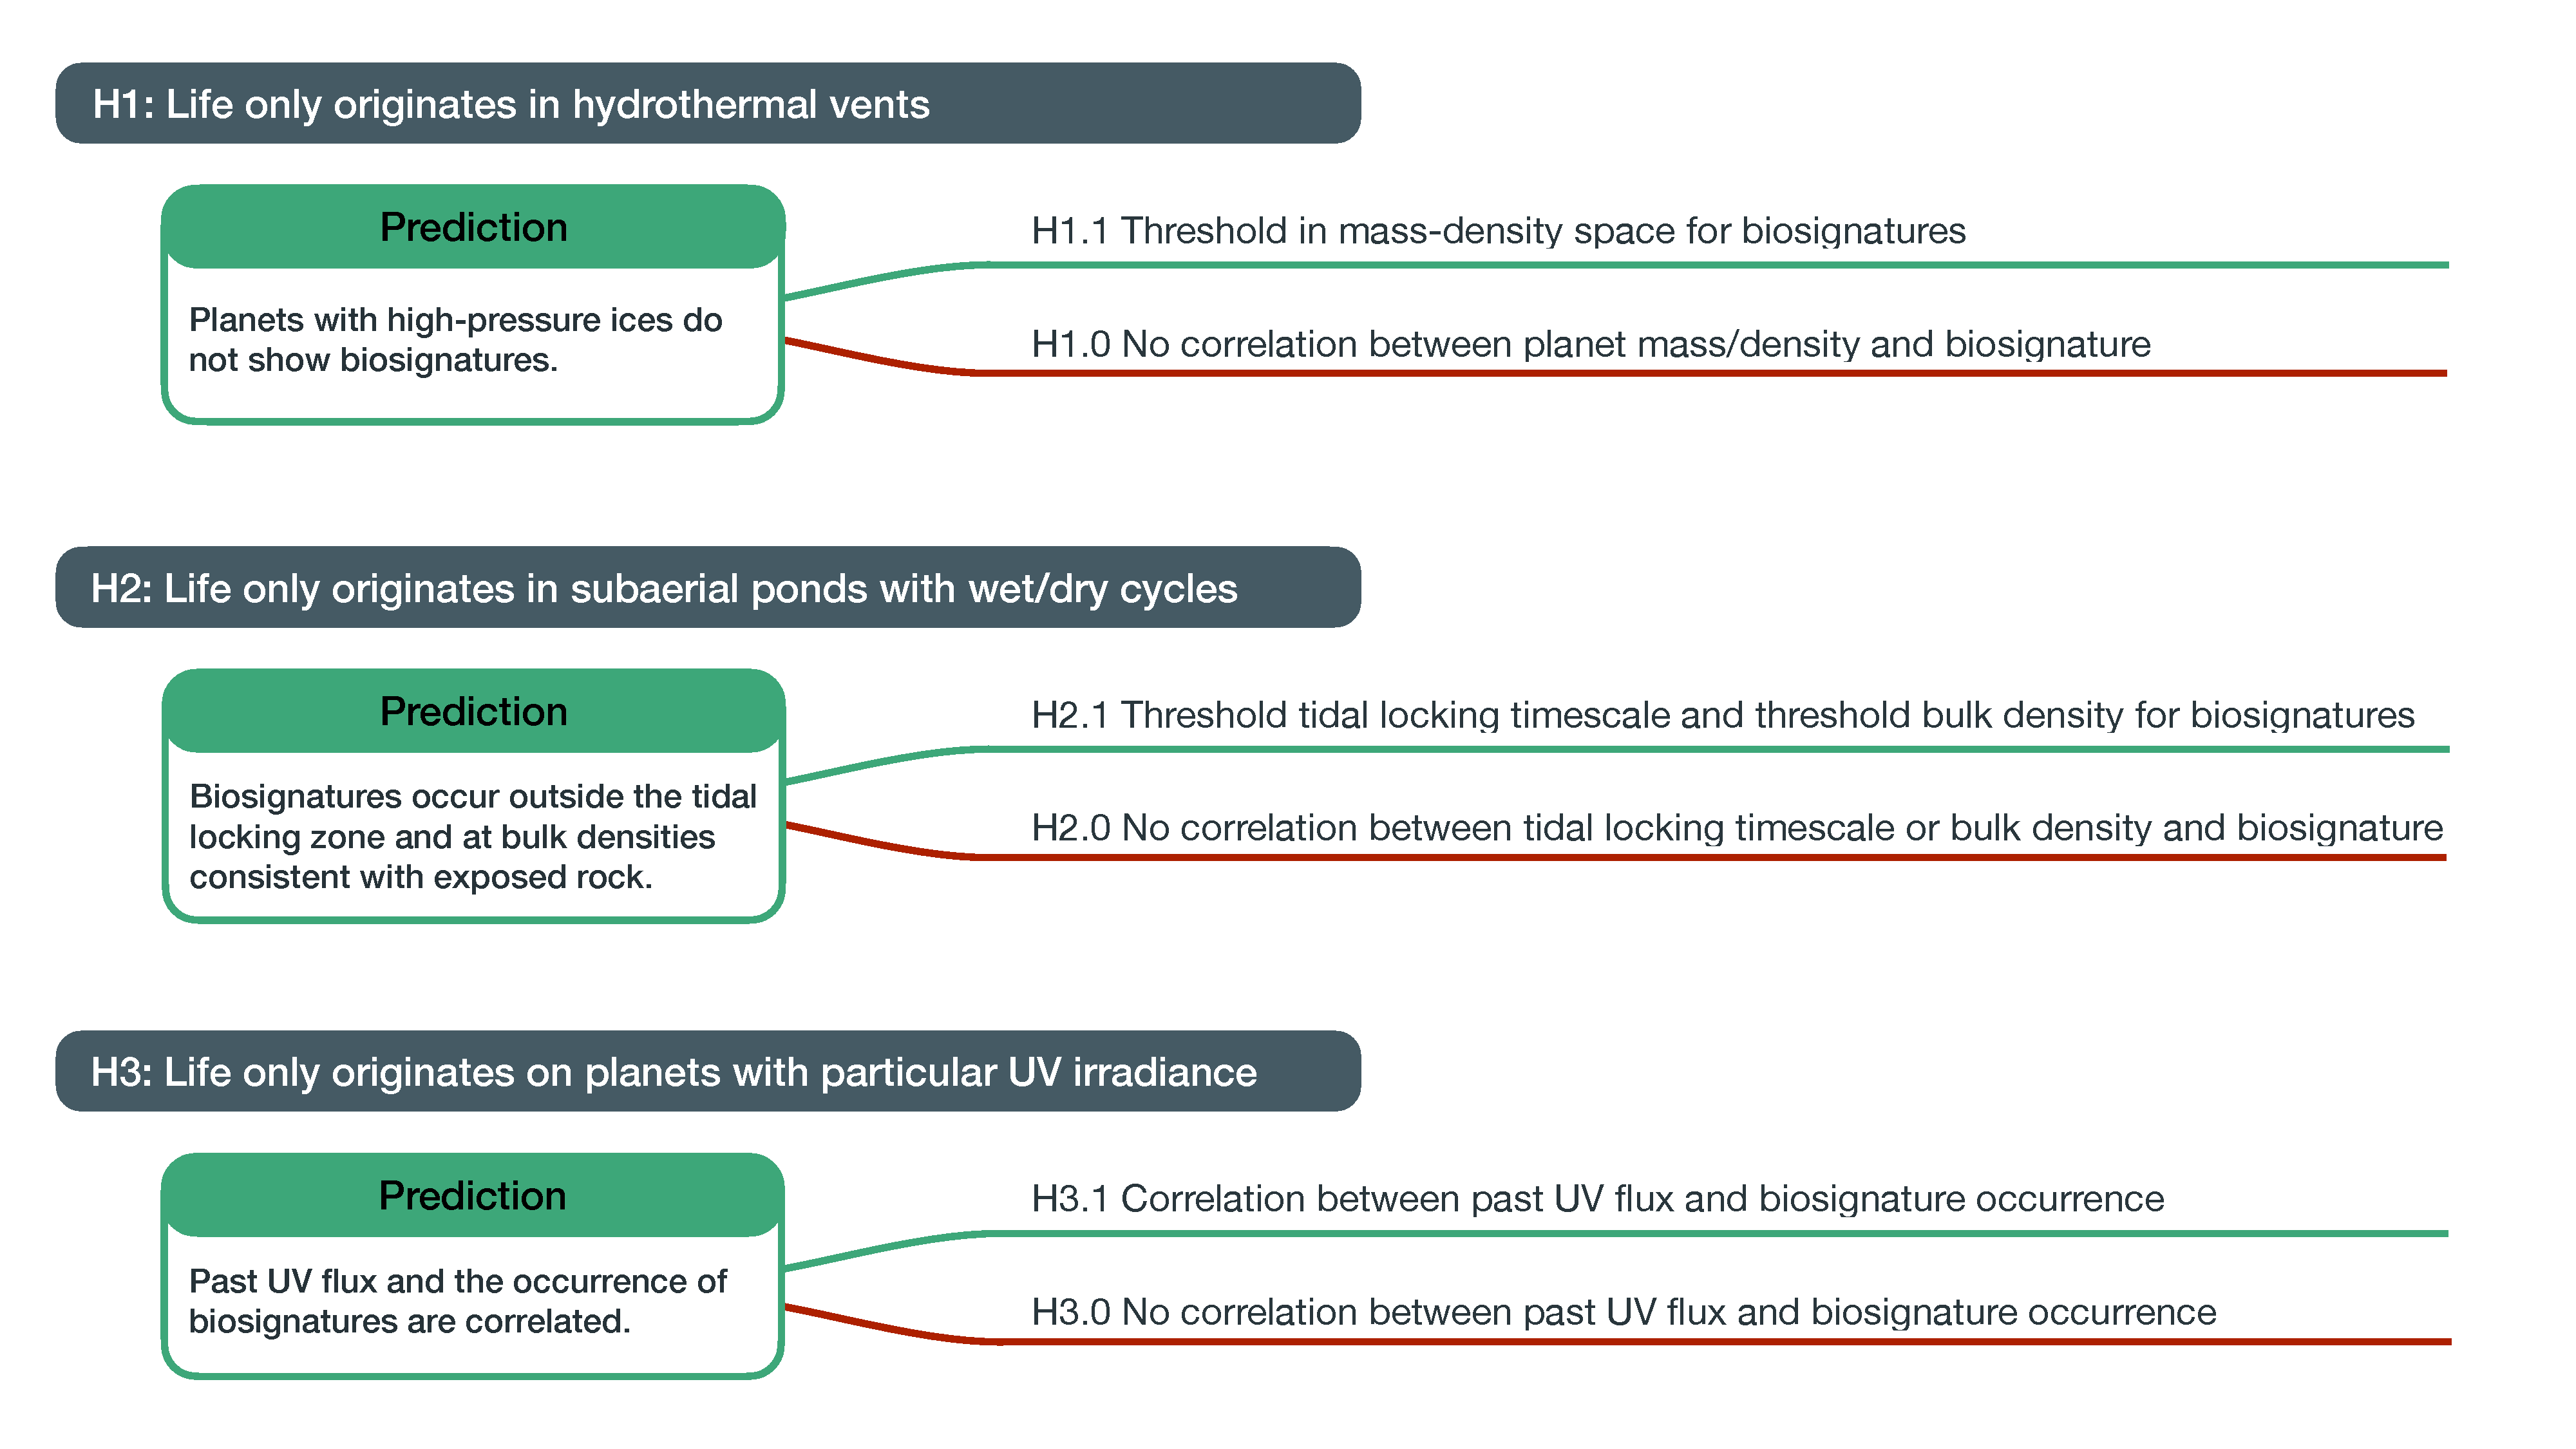
\includegraphics[width=\hsize]{figures/hypotheses.pdf}
        \caption{Origins of Life scenarios, their predictions on exoplanet observables, and derived population-level hypotheses.}
        \label{fig:hypotheses}
    \end{centering}
\end{figure*}
Figure~\ref{fig:hypotheses} lists the hypotheses derived from the predictions of each OOL scenario.
...


\section{Hypothesis Tests}
\label{sec:hypotests}
\todo[inline]{Briefly introduce Bayesian model comparison, then present the particular hypotheses in their mathematical form.}

\subsection{Habitable Zone}
All Origins of Life scenarios considered here require water as a solvent; we thus consider only planets that may sustain liquid water on their surface.
Different formulations of habitable zones as regions around a star where a planet with Earth's atmospheric composition can maintain liquid water on its surface exist~\citep[e.g.,][]{MolLous2022,Spinelli2023,Tuchow2023}. CITE! Ramirez \& Kaltenegger 2017, 2018
Here, we adopt the popular estimates of \citet{Kasting1993} and \citet{Kopparapu2013,Kopparapu2014} that define a temperate zone between the runaway greenhouse transition CITE! and the maximum greenhouse limit CITE!.
We use the parametrization in \citet{Kopparapu2014} to derive luminosity and planetary mass-dependent edges of the habitable zone $a_\mathrm{inner}$ and $a_\mathrm{outer}$.


\subsection{Bayesian hypothesis testing with \bioverse}

\subsection{H1: Life only originates in hydrothermal vents}
The hydrothermal vent scenario does not allow oceans deep enough to form an impenetrable layer of high-pressure ice on its floor.
The resulting allowed parameter space is described by a lower limit on the bulk density. \todo[inline]{+ exclude atmospheric signature for water worlds?}
...

\subsection{H2: Life only originates in subaerial ponds with wet/dry cycles}
We parametrize the required exposed land surface in this scenario as a lower limit in bulk density that is higher than for H1.
Further, the tidal locking timescale of the planet may not be smaller than the age of the system.
...

\subsection{H3: Life only originates on planets with particular UV irradiance}
We test a UV irradiance requirement by relating the occurrence of life on a planet with a minimum past UV flux, which is a function of ...? \todo[inline]{SUKRIT}

\todo[inline]{OPTIONAL: ``We further test the scenario of a linear correlation of past UV flux and biosignature occurrence rate.
This test requires the detection of multiple biosignatures.''
~\\
Test for negative correlations as well?}


\section{Exoplanet survey simulations}
\todo[inline]{biomarkers: Focus on molecular Oxygen? Excess Methane? \citep[e.g.,][]{Seeburger2023}}
A commonly discussed biomarker is molecular Oxygen (O$_2$), which on Earth emerged as a byproduct of photosynthesis during the Proterozoic era.
While not the only atmospheric species discussed as a signature for planetary life CITE, we focused on O$_2$ as a representative biomarker for our spectroscopic survey simulations.


\subsection{Habitable Worlds Observatory}
\subsubsection{target list}
\todo[inline]{Provisional stellar target List for the habitable Worlds Observatory:~\citep{Mamajek2023}}


\subsection{Nautilus}
\subsection{LIFE} % optional


\section{Results}
\label{sec:results}
\subsection{Information content in mass-density space}

\subsection{Information content in tidal locking timescale-density space}

\subsection{Correlation of past UV flux and biosignature occurrence}

\section{Discussion and Conclusions}
\label{sec:discussion}
%''Which natural processes best explain how living matter spontaneously appears from nonliving matter?''~\citep{Malaterre2022}
%WE consider life ``as we know it''

\subsection{What do we learn from a single biosignature detection?}
\todo[inline]{discuss constraining power on OOL of a convincing biosignature detection on a single planet, depending on the position of the planet in the parameter space we explored.}

\subsection{Constraining power for the origins of life as a function of biosignature location}
\todo[inline]{How does the location of biosignature detections impact the credibility of OOL scenarios?}
\todo[inline]{biosignature on M~dwarf planet vs. FGK: Impact on UV flux requirement?}

\subsection{Caveats}
\subsubsection{Atmosphere transmission}
Theoretical work suggests that the atmosphere of prebiotic Earth was largely transparent at near-UV wavelengths with the only known source of attenuation being Rayleigh scattering~\citep{Ranjan2017,Ranjan2017c}.
We thus approximated surface UV flux using top-of-atmosphere fluxes.
This represents a conservative approach, since any planet that fails to meet the irradiance criterion receives even lower near-UV radiation at its surface. \todo[inline]{SUKRIT please specify as neccessary}

\subsubsection{Stellar flares}
Our assumptions on past UV flux neglect the contribution of stellar flares, which may be hypothesized as an alternative source of UV light~\citep{Ranjan2017}.
This concerns mainly ultracool dwarfs, due to their low quiescent emission and high pre-main sequence stellar activity~\citep{Buccino2007,West2008}.
Recent work indicates that the majority of stars show inadequate activity levels for a sufficient contribution through flares~\citep{Glazier2020,Ducrot2020,Günther2020}.
The biosignature surveys we simulated here may test the hypothesis of sufficient UV radiation via stellar flares.




\subsection{Conclusions and future work}

%\begin{acknowledgments}
\section*{Acknowledgments}
    The authors thank Kevin Heng, Dominik Hintz, Chia-Lung Lin, and Rhys Seeburger for insightful discussions.
%    We are grateful to ...
%    mention any people who gave comments in early-on meetings
    We thank the anonymous referee for providing constructive critical feedback that helped to improve this manuscript.
    This material is based upon work supported by the National Aeronautics and Space Administration under Agreement No. 80NSSC21K0593 for the program ``Alien Earths''.
    The results reported herein benefited from collaborations and/or information exchange within NASA’s Nexus for Exoplanet System Science (NExSS) research coordination network sponsored by NASA’s Science Mission Directorate.
    This work has made use of data from the European Space Agency (ESA) mission \gaia\ (\url{https://www.cosmos.esa.int/gaia}), processed by the \gaia\ Data Processing and Analysis Consortium (DPAC, \url{https://www.cosmos.esa.int/web/gaia/dpac/consortium}). Funding for the DPAC has been provided by national institutions, in particular the institutions participating in the \gaia\ Multilateral Agreement.
    T.L. was supported by the Branco Weiss Foundation, the Netherlands eScience Center (PROTEUS project, NLESC.OEC.2023.017), and the Alfred P. Sloan Foundation (AEThER project, G202114194).
%    ...
\end{acknowledgments}

\section*{Author contributions}
M.S., D.A., and S.R.\ conceived the project, planned its implementation, and interpreted the results.
M.S.\ developed the planetary evolution component to \bioverse, carried out the hypothesis tests and statistical analyses, and wrote the manuscript.
D.A.\ leads the ``Alien Earths'' program through which this project is funded, helped to guide the strategy of the project, and provided text contributions.
A.A.\ carried out the semi-analytical computations regarding the correlation of past UV flux and biosignature occurrence.
S.R.\ advised on planetary \gls{NUV} flux evolution and the cyanosulfidic scenario of the origins of life.
R.F.\ wrote the initial draft of the Introduction and advised on the evolutionary biology aspects of the project.
K.H.-U.\ contributed to the \bioverse\ software development and simulations.
%M.S.\ wrote the manuscript; ... and ... provided text contributions.
T.L.\ supported the selection of testable hypotheses and provided text contributions to the initial draft.
S.M.\ advised on the scope of the project and supported the selection of testable hypotheses.
All authors provided comments and suggestions on the manuscript.


%Author affiliations (tbd):
%Martin Schlecker1, Daniel Apai1,2, Antonin Affholder4, Sukrit Ranjan2, Regis Ferriere4, Kevin Hardegree-Ullman1, Tim Lichtenberg3, and Stephane Mazevet5
%1 Steward Observatory and Department of Astronomy, The University of Arizona, Tucson, AZ 85721, USA
%2 Lunar and Planetary Laboratory, The University of Arizona, Tucson, AZ 85721, USA
%3 Kapteyn Astronomical Institute, University of Groningen, PO Box 800, 9700 AV Groningen, The Netherlands
%4 Department of Ecology and Evolutionary Biology, University of Arizona, Tucson, AZ, USA
%5 Observatoire de la Côte d’Azur, 96 Boulevard de l’Observatoire, F-06300 Nice, France


\section*{Reproducibility}

\bibliography{bib,coauthors}

\end{document}
